\documentclass[14pt,a4paper,fleqn]{extarticle}
\usepackage[T2A,T1]{fontenc}
\usepackage[utf8]{inputenc}
\usepackage[russian]{babel}
\usepackage{amsmath}
\usepackage{graphicx}
\usepackage{tabularx}
\usepackage{boldline}
\usepackage{makecell}
\usepackage{arydshln}
\usepackage{mathtools}

\graphicspath{ {./images/} }
\setlength{\mathindent}{0pt}
\setlength\parindent{0pt}


\begin{document}
	\begin{titlepage}
		
\includegraphics[scale=0.12]{logo}
		\begin{center}
			\textbf{МИНОБРНАУКИ РОССИИ}\\
			\vspace{0.2cm}
			\textbf{Федеральное государственное бюджетное образовательное учреждение высшего образования}\\
			\textbf{«САНКТ-ПЕТЕРБУРГСКИЙ ГОСУДАРСТВЕННЫЙ ЭКОНОМИЧЕСКИЙ УНИВЕРСИТЕТ»}\\
			\vspace{0.6cm}
			Факультет информатики и прикладной математики\\
			Кафедра прикладной математики и экономико-математических методов\\
			\vspace{1cm}
			\textbf{ОТЧЁТ}\\
			по дисциплине:\\
			\textbf{«Методы оптимизации»}\\
			на тему:\\
			\textbf{«Решение задачи дискретной оптимизации методом ветвей и границ. Задание 10»}\\
		\end{center}
		\vspace{1cm}
		Направление: 01.03.02\\
		Обучающийся: Бронников Егор Игоревич\\
		Группа: ПМ-1901\\
		\vfill
		\begin{center}
			Санкт-Петербург\\
			2021\\
		\end{center}
	\end{titlepage}
	\section*{Задача 4}
	Целевая функция:\\
	$f = 4x_1+x_2 \longrightarrow max$\\\\
	Ограничения:
	\begin{align*}
		\begin{cases}
			3x_1 - 2x_2 \geq -8\\
			3x_1 + x_2 \geq 3\\
			x_2 \leq 8\\
			x_1 \leq 4\\
		\end{cases}
	\end{align*}
	$x_1 \geq 0, x_2 \geq 0$\\
	
	Оптимальное решение задачи:\\
	$f = 24, x_1 = 4, x_2 = 8$\\
	Решение исходной задачи получилось целочисленным, поэтому её нужно испортить.\\
	
	\textbf{Испортим исходную задачу:}\\
	
	Целевая функция:\\
	$f = 4x_1+x_2 \longrightarrow max$\\\\
	Ограничения:
	\begin{align*}
		\begin{cases}
			3x_1 - 2x_2 \geq -8\\
			3x_1 + x_2 \geq 3\\
			\boldsymbol{5} x_2 \leq 8\\
			\boldsymbol{3} x_1 \leq 4\\
		\end{cases}
	\end{align*}
	$x_1 \geq 0, x_2 \geq 0$\\
	
	Оптимальное решение испорченной задачи:\\
	$f = 6.93333, x_1 = 1.33333, x_2 = 1.6$
	\newpage
	
	В качестве переменной для ветвления возьмём переменную $x_1$. Разобьём исходну задачу на две подзадачи 1.1 и 1.2.
	\subsection*{Задача 1.1}
	Добавляем ограничение: $x_1 \geq 2$.\\
	
	Целевая функция:\\
	$f = 4x_1+x_2 \longrightarrow max$\\\\
	Ограничения:
	\begin{align*}
		\begin{cases}
			3x_1 - 2x_2 \geq -8\\
			3x_1 + x_2 \geq 3\\
			5 x_2 \leq 8\\
			3 x_1 \leq 4\\
			x_1 \geq 2\\
		\end{cases}
	\end{align*}
	$x_1 \geq 0, x_2 \geq 0$\\
	
	Так получилось, что данная задача не имеет решения, поэтому для неё процесс ветвления прерывается.
	\newpage
	\subsection*{Задача 1.2}
	Добавляем ограничение: $x_1 \leq 1$.\\
	
	Целевая функция:\\
	$f = 4x_1+x_2 \longrightarrow max$\\\\
	Ограничения:
	\begin{align*}
		\begin{cases}
			3x_1 - 2x_2 \geq -8\\
			3x_1 + x_2 \geq 3\\
			5 x_2 \leq 8\\
			3 x_1 \leq 4\\
			x_1 \leq 1\\
		\end{cases}
	\end{align*}
	$x_1 \geq 0, x_2 \geq 0$\\
	
	Оптимальное решение данной задачи:\\
	$f = 5.6, x_1 = 1, x_2 = 1.6$\\
	
	Опять получили нецелочисленное решение и разбиваем задачу 1.2 на две задачи 1.2.1 и 1.2.2.
	\newpage
	\subsection*{Задача 1.2.1}
	Добавляем ограничение: $x_2 \geq 2$.\\
	
	Целевая функция:\\
	$f = 4x_1+x_2 \longrightarrow max$\\\\
	Ограничения:
	\begin{align*}
		\begin{cases}
			3x_1 - 2x_2 \geq -8\\
			3x_1 + x_2 \geq 3\\
			5 x_2 \leq 8\\
			3 x_1 \leq 4\\
			x_1 \leq 1\\
			x_2 \geq 2\\
		\end{cases}
	\end{align*}
	$x_1 \geq 0, x_2 \geq 0$\\
	Так получилось, что данная задача не имеет решения, поэтому для неё процесс ветвления прерывается.\\
	\newpage
	\subsection*{Задача 1.2.2}
	Добавляем ограничение: $x_2 \leq 1$.\\
	
	Целевая функция:\\
	$f = 4x_1+x_2 \longrightarrow max$\\\\
	Ограничения:
	\begin{align*}
		\begin{cases}
			3x_1 - 2x_2 \geq -8\\
			3x_1 + x_2 \geq 3\\
			5 x_2 \leq 8\\
			3 x_1 \leq 4\\
			x_1 \leq 1\\
			x_2 \leq 1\\
		\end{cases}
	\end{align*}
	$x_1 \geq 0, x_2 \geq 0$\\
	
	Оптимальное решение данной задачи:\\
	\underline{$f = 5, x_1 = 1, x_2 = 1$}\\
	
	Получили первое целочисленное решение данной задачи.\\
	
	Теперь в качестве переменной для ветвления возьмём переменную $x_2$. Разобьём исходну задачу на две подзадачи 2.1 и 2.2.
	\newpage
	\subsection*{Задача 2.1}
	Добавляем ограничение: $x_2 \geq 2$.\\
	
	Целевая функция:\\
	$f = 4x_1+x_2 \longrightarrow max$\\\\
	Ограничения:
	\begin{align*}
		\begin{cases}
			3x_1 - 2x_2 \geq -8\\
			3x_1 + x_2 \geq 3\\
			5 x_2 \leq 8\\
			3 x_1 \leq 4\\
			x_2 \geq 2\\
		\end{cases}
	\end{align*}
	$x_1 \geq 0, x_2 \geq 0$\\
	
	Так получилось, что данная задача не имеет решения, поэтому для неё процесс ветвления прерывается.\\
	
	\newpage
	\subsection*{Задача 2.2}
	Добавляем ограничение: $x_2 \leq 1$.\\
	
	Целевая функция:\\
	$f = 4x_1+x_2 \longrightarrow max$\\\\
	Ограничения:
	\begin{align*}
		\begin{cases}
			3x_1 - 2x_2 \geq -8\\
			3x_1 + x_2 \geq 3\\
			5 x_2 \leq 8\\
			3 x_1 \leq 4\\
			x_2 \leq 1\\
		\end{cases}
	\end{align*}
	$x_1 \geq 0, x_2 \geq 0$\\
	
	Оптимальное решение данной задачи:\\
	$f = 6.33333, x_1 = 1.33333, x_2 = 1$\\
	Опять получили нецелочисленное решение и разбиваем задачу 2.2 на две задачи 2.2.1 и 2.2.2.
	\newpage
	\subsection*{Задача 2.2.1}
	Добавляем ограничение: $x_1 \geq 2$.\\
	
	Целевая функция:\\
	$f = 4x_1+x_2 \longrightarrow max$\\\\
	Ограничения:
	\begin{align*}
		\begin{cases}
			3x_1 - 2x_2 \geq -8\\
			3x_1 + x_2 \geq 3\\
			5 x_2 \leq 8\\
			3 x_1 \leq 4\\
			x_2 \leq 1\\
			x_1 \geq 2\\
		\end{cases}
	\end{align*}
	$x_1 \geq 0, x_2 \geq 0$\\
	
	Так получилось, что данная задача не имеет решения, поэтому для неё процесс ветвления прерывается.\\
	\newpage
	\subsection*{Задача 2.2.2}
	Добавляем ограничение: $x_1 \leq 1$.\\
	
	Целевая функция:\\
	$f = 4x_1+x_2 \longrightarrow max$\\\\
	Ограничения:
	\begin{align*}
		\begin{cases}
			3x_1 - 2x_2 \geq -8\\
			3x_1 + x_2 \geq 3\\
			5 x_2 \leq 8\\
			3 x_1 \leq 4\\
			x_2 \leq 1\\
			x_1 \leq 1\\
		\end{cases}
	\end{align*}
	$x_1 \geq 0, x_2 \geq 0$\\
	
	Оптимальное решение данной задачи:\\
	\underline{$f = 5, x_1 = 1, x_2 = 1$}\\
	
	Получили второе целочисленное решение данной задачи, которое совпало с первым.\\
	
	\textbf{Ответ:} $f = 5, x_1 = 1, x_2 = 1$
	\newpage
	\subsection*{Процесс ветвления}
	\subsubsection*{По переменной $x_1$}
	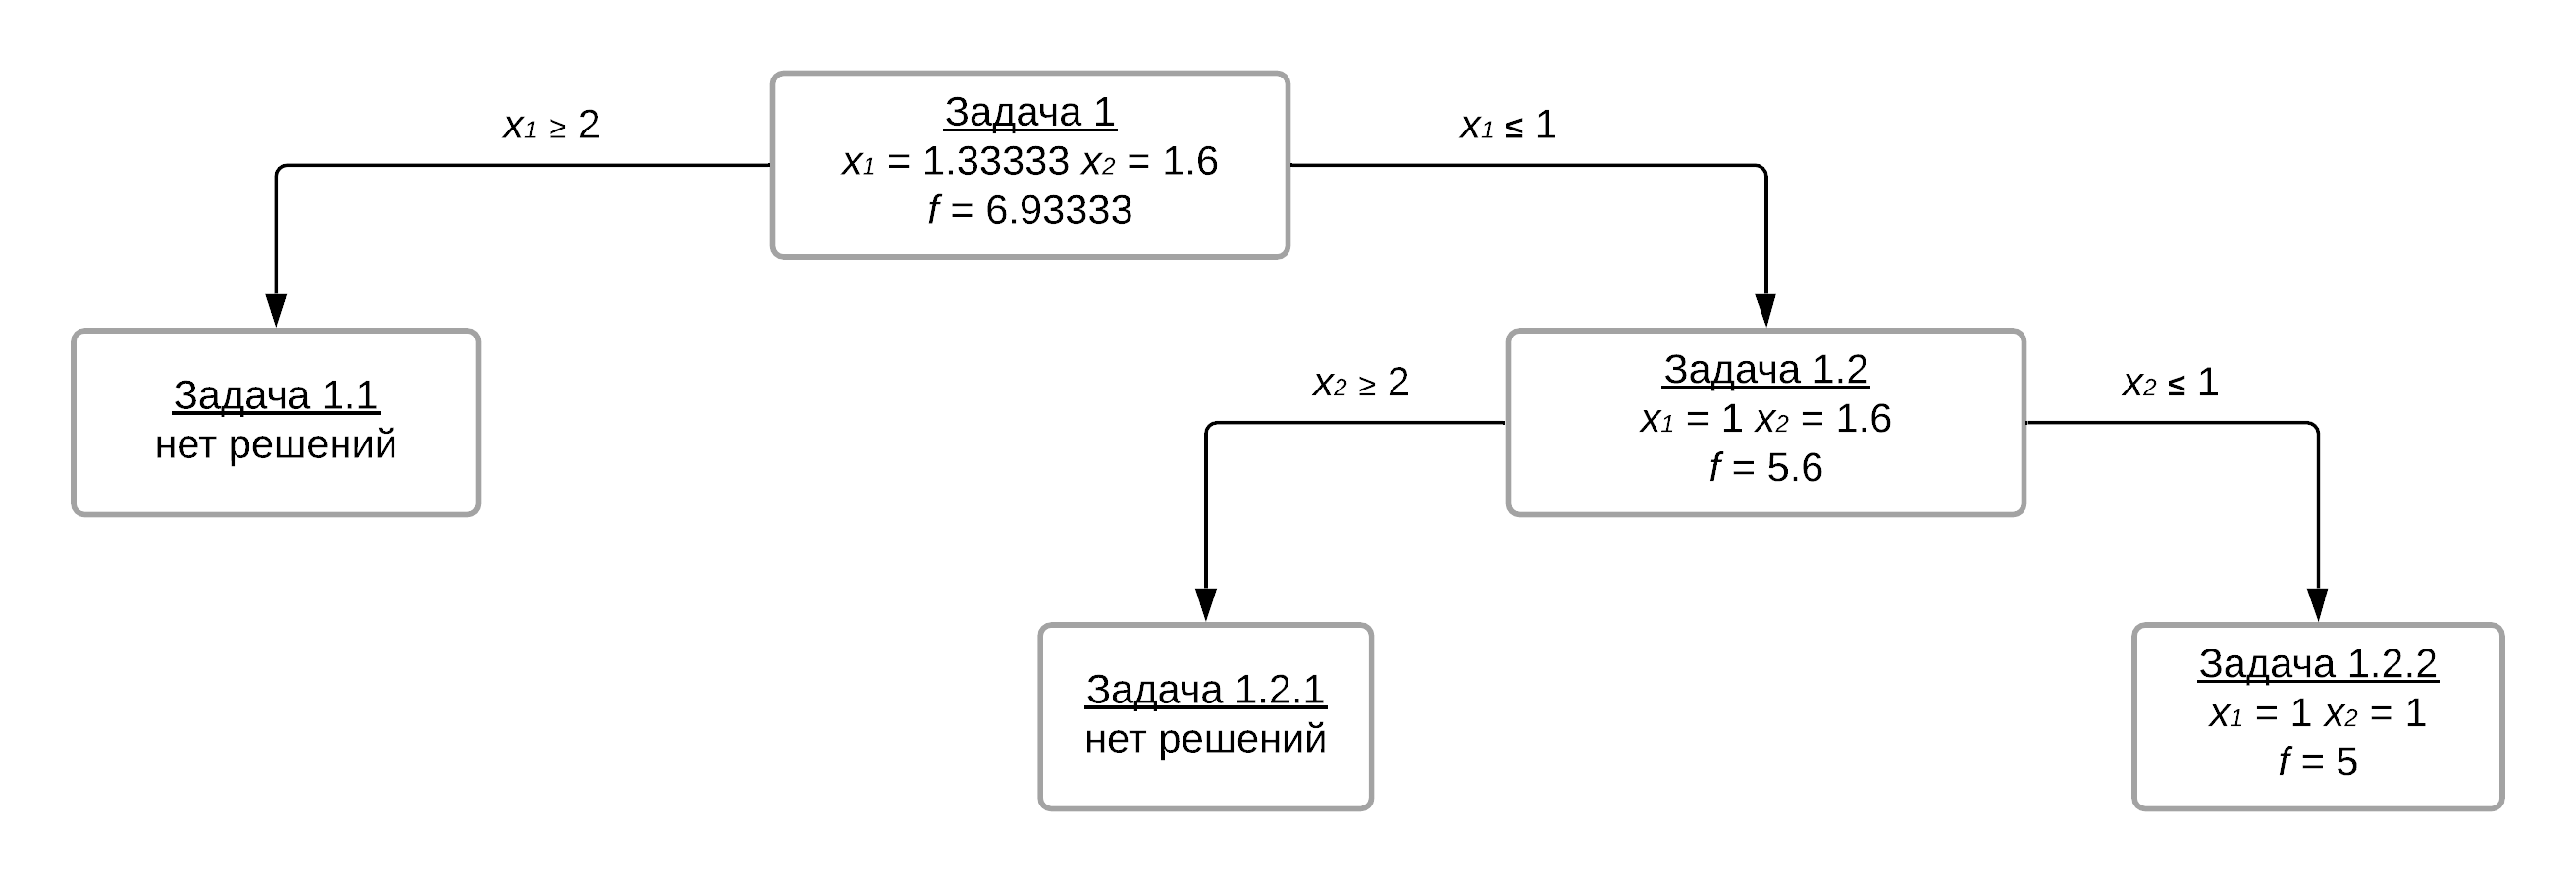
\includegraphics[scale=0.18]{1}
	\subsubsection*{По переменной $x_2$}
	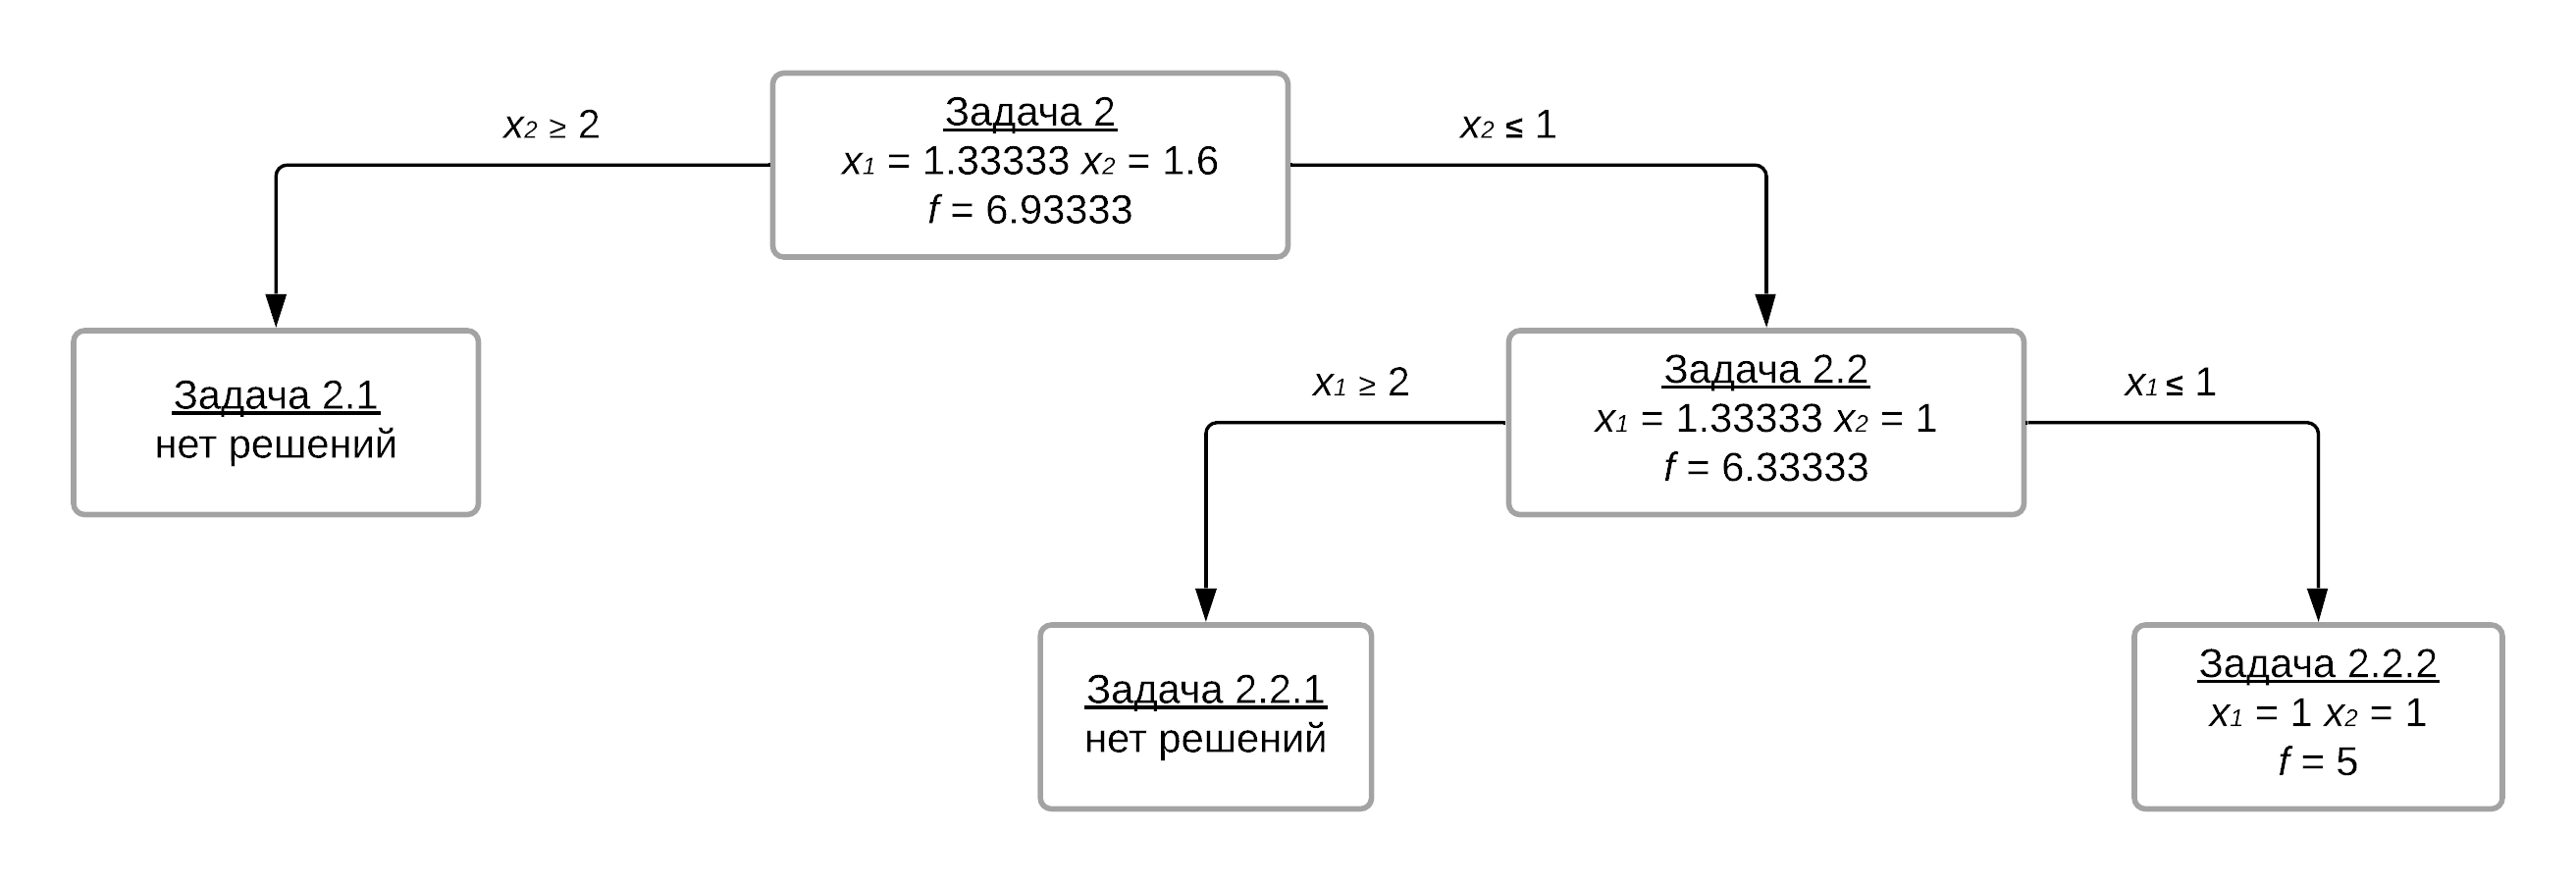
\includegraphics[scale=0.18]{2}
\end{document}